\documentclass{hw}
\title{Programming Assignment 3:\\ Semantic Analysis}

\usepackage{fancyvrb}
\usepackage{mathpartir}
\usepackage{pervasives}
\usepackage{tikz}
\usetikzlibrary{positioning}

\begin{document}
\maketitle

\section{Metadata}\label{sec:metadata}
% The fully qualified class name of your main program and any other
% instructions needed to run the program.
We implemented programming assignment $1$ and $2$ in Java, but we implemented
programming assignment $3$ in OCaml. Our main OCaml executable is implemented
in \texttt{main.ml} inside the \texttt{src} directory. To run our code, you
will need to install a couple of packages and OCaml libraries by running the
following:

\begin{center}
\begin{BVerbatim}
sudo apt-get install aspcud m4 unzip
opam install core async oUnit
\end{BVerbatim}
\end{center}

To build our executable, simply run \texttt{make src}. This will use
\texttt{jflex}, \texttt{cup}, and \texttt{javac} and build all of our Java
code. It will use \texttt{corebuild} to build our OCaml code.  Invoking our
code manually is hard; instead, we we recommend you use the \texttt{xic} script
which invokes our code with everything configured properly.

In summary, perform the following:

\begin{center}
\begin{BVerbatim}
sudo apt-get install aspcud m4 unzip
opam install core async oUnit
make src
./xic [flags] <xi_file.xi>...
\end{BVerbatim}
\end{center}

\section{Summary}\label{sec:summary}
In this programming assignment, we implemented semantic analysis in OCaml for
the Xi programming language. Our largest design decisions involve switching to
OCaml and the format of our AST. The most challenging aspect of the assignment
was the handling of the empty array. There are no known problems with our
implementation.

\section{Specification}\label{sec:specification}
In this section, we make explicit our interpretation of the Xi language
specification and discuss various language extensions we have implemented.

\subsection{Assignment to Underscore}
This is one of the released test cases:
%
\begin{verbatim}
main() {
    _ = 2;
}
\end{verbatim}
%
The test harness expects us to throw an error saying that a function call was
expected. We \emph{intentionally} fail this test case and allow this construct.
We think disallowing this construct is somewhat arbitrary and makes it unclear
when an underscore is allowed and when it is not. We allow underscores almost
everywhere you expect a variable declaration.

One may argue that a function call is the only sane thing to have on the right
hand side of an assignment to underscore because it is the only thing that has
side effects. However, this is not strictly true. We could nest a function in
another expression (e.g. \texttt{\_ = 1 + f()}). We may want to run multiple
functions and disregard all of them like this: \texttt{\_ = \{f(); g(); h()\}}.
Maybe, we want to check that a function returns an array of at least one
element: \texttt{\_ = f()[0]}. Maybe we want to crash the program: \texttt{\_ = 1
/ 0} or \texttt{\_ = \{\}[0]}. We feel there are many reasons why you would want
to throw away expressions that are not functions.

If you really, really feel strongly about us disallowing this, then open up
\texttt{typecheck.ml} and grep for \texttt{COMPILERS IS FUN}. Then, uncomment
out the code that is there; this will disallow non-function call assignments to
underscore.

\subsection{Annotated Underscore}
In the same spirit as above, we allow annotated underscores like \texttt{\_:int
= 1}. This allows a programmer to assert the return types of functions:
\texttt{\_:int = f(); \_:bool = g()}.

\subsection{Multiple Declarations}
We allow multiple declarations without assignment (e.g. \texttt{x:int,
y:bool}). This makes single and multiple declarations more consistent and is
rather useful to do.

\subsection{Empty Arrays}
We handle empty arrays pretty liberally. For example, all of the following are
well-typed according to us.
\begin{verbatim}
_:int[] = {}
_:int[][] = {{}, {1}, {}}
_:bool[][] = {{}, {true}, {}}
_:bool[][] = {{}, {true}, {}} + {}
_:bool[][] = {{}, {true}, {}} + {} + {{}}
_:bool[][] = length({})
\end{verbatim}
One of the few things we disallow is indexing into an empty array literal,
which is erroneous anyway. We do this by introducing additional production
rules to our subtype relation to handle empty arrays which we give a special
type: \texttt{empty}
\begin{mathpar}
  \inferrule
  { }
  {\texttt{empty} \leq \tau\texttt{[]}}

  \inferrule
  {\tau_1 \leq \tau_2}
  {\tau_1\texttt{[]} \leq \tau_2\texttt{[]}}
\end{mathpar}

\section{Design and Implementation}\label{sec:design}
\subsection{Architecture}
\begin{figure}[h]
  \centering
  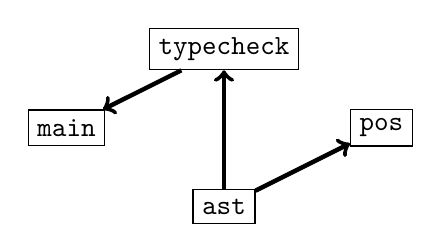
\begin{tikzpicture}
    \tikzstyle{every node}+=[draw]
    \node (main)  at (0, 0)  {\texttt{main}};
    \node (typecheck) at (2, 1)  {\texttt{typecheck}};
    \node (ast)   at (2, -1) {\texttt{ast}};
    \node (pos)   at (4, 0)  {\texttt{pos}};
    \path[->, ultra thick] (ast)   edge (pos)
                           (ast)   edge (typecheck)
                           (typecheck) edge (main);
  \end{tikzpicture}
  \caption{%
    Module Dependency Diagram. Each node represents a module. An arrow from
    module $u$ to module $v$ signifies that $v$ depends on $u$.
  }
  \label{fig:mdd}
\end{figure}

We had four main files in our typechecker, as shown in \figref{mdd}.
\begin{enumerate}
  \item{\texttt{main.ml}:}
    This is the main front end for our compiler. In this class, we handle the
    various command line options passed into the binary and call the rest of
    our lexing, parsing, and typechecking code. We also handle all IO (including the typechecking
    output) in this class.

  \item{\texttt{typecheck.ml}:}
    This file contains the typechecking logic and implements the interface defined by \texttt{typecheck.mli}.
    
  \item{\texttt{ast.ml}:}
    This file is similar to Ast.java for \texttt{pa2} except that we utilize OCaml. We define our AST nodes by using OCaml abstract data types.

  \item{\texttt{pos.ml}:}
    This class represents a position (row and column) and contains many helpful helper functions that construct expressions and statements without worrying about the position.

\end{enumerate}

\subsection{Code Design}
One of the main extensions we implemented was in comments. The project
specification states that comments were only to be terminated by a newline, but
we allowed comments that were terminated by any line terminals (\verb$\r$,
\verb$\r\n$, and \verb$\n$) and by EOF.  We added the EOF case since it is
conceivable that programmers would end a source file with a comment, and having
a lexing failure in this case would be undesireable.

\newcommand{\minint}{9223372036854775808}
\newcommand{\maxint}{9223372036854775807}
Another design decision revolved around the lexing of integer literals. In Xi,
integer literals fall in the range of $[-2^{63}, 2^{63}-1] = [-\minint,
\maxint]$. A peculiarity arises when lexing the string $s = $
\texttt{-\minint}. If a lexer parses $s$ as two tokens: a minus sign and an
integer literal, the integer literal $\minint$ is too large to be a valid
integer literal. This can be solved with regular expressions, though this
solution is inelegant. Instead, we introduce a new \texttt{BIG\_NUM} token
which is generated by the occurrence of \texttt{\minint}. We then defer the
responsibility of ensuring a \texttt{BIG\_NUM} token is preceded by a minus
token to the parser.

We also added extensive lexical error support by way of our
\texttt{XicException} class. While the examples only gave the empty character
exception, we added several other error cases, such as out of bounds long
literals, invalid hex literals, unterminated strings and character literals,
and invalid tokens (a catch-all for symbols unsupported in the language
specification).

\subsection{Programming}
We implemented our lexer using both a bottom-up and a top-down approach. Some
members of our team used a bottom-up approach to implement our
\texttt{XicException} exception class and \texttt{Sym} symbol class---both
of which do not depend on any other class---without knowing exactly how they
would be used by other classes. Conversely, other members implemented our
\texttt{Main} class without yet knowing the specific implementation of the
underlying lexer. We also followed the designed principle of test driven
development, implementing tests cases as we implemented our lexer to catch bugs
often and early. This is described in detail in \secref{testing}.

We encountered various issues while implementing our lexer, most of which
revolved around the subtle interactions between whitespace characters and
regular expressions that are more complicated than they seem. The most
obnoxious issue revolved around the following regular expression we initially
used to match comments.

\begin{center}
\begin{BVerbatim}
LineTerminator = \n | \r | \r\n
Comment = "//" (!{LineTerminator})* {LineTerminator}
\end{BVerbatim}
\end{center}

Intuitively, the \texttt{Comment} regular expression matches \texttt{//}, any
number of characters that aren't \verb$\r$, \verb$\n$, or \verb$\r\n$, and
finally a line terminator. Surprisingly though, the string \verb$//a\r\na\n$ is
lexed as a single comment, not as a comment and then an identifier \verb$a$!
Inspecting the regular expression deeper, we see the language of
\verb${Comment}$ is \verb${\r, \n, \r\n}$. The language of \verb$!{Comment}$ is
then everything that's not in \verb${\r, \n, \r\n}$. This set includes
\verb$a\r$ and \verb$\na$! Thus, \verb$a\r\na$ is matched by
\verb$(!{LineTerminator})*$.

The distribution of work is described in detail in \secref{workplan}.

\section{Testing}\label{sec:testing}
We wrote numerous JUnit tests to verify the correctness of our lexer. We
started with very basic tests that would test one token at a time. Then, we
moved on to more complex tests where we would mix up different tokens or add
random white spaces before, after or between the tokens. After that we created
more test cases with escape characters, line terminators and EOF. Lastly, we
created invalid tests to make sure that we are throwing the correct exceptions.

Our test plan worked out very well. First testing on very basic tokens helped
us solidify the majority of our code. Then, testing with escape characters and
line terminators helped us find a lot of bugs in our code and made sure that we
were dealing with white spaces correctly.  Finally, testing that exceptions
were thrown properly again made sure we covered all the corner cases in our
lexer.

\section{Work Plan}\label{sec:workplan}
Before we started coding, one person set up the skeleton code and
modularization. Then another member took care of the frontend such as command
line interfaces. Then, other people wrote the rules for lexing while the other
members wrote test cases.

\section{Known Problems}\label{sec:problems}
None.

\section{Comments}\label{sec:comments}
We spent about 60 hours total on the assignment. The assignment overall
introduced important concepts about lexing but we thought the coding was a
little bit dry and tedious.

\end{document}
